\documentclass{article}
\usepackage{../fasy-hw}

%% UPDATE these variables:
\renewcommand{\hwnum}{3}
\title{Computational Topology, Homework \hwnum}
\author{\todo{your name here}}
\collab{\todo{list your collaborators here}}
\date{due: 3 March 2022 (accepted through 7 March 2022)}

\begin{document}

\maketitle

This homework assignment should be submitted as a single PDF file to D2L.

General homework expectations:
\begin{itemize}
    \item Homework should be typeset using LaTex.
    \item Answers should be in complete sentences, and make sense without
        seeing the question.
    \item You will not plagiarize, nor will you share your written solutions
        with classmates.  (But, discussing the questions is highly encouraged).
    \item List collaborators at the start of each question using the
        \texttt{collab} command.
    \item Put your answers where the \texttt{todo} command currently is (and
        remove the \texttt{todo}, but not the word \texttt{Answer}).
    \item If you are asked to come up with an algorithm, you are
        expected to give an algorithm that beats the brute force (and, if possible, of
        optimal time complexity). With your algorithm, please provide the following:
        \begin{itemize}
            \item \emph{What}: A prose explanation of the problem and the algorithm,
                including a description of the input/output.
            \item \emph{How}: Describe how the algorithm works, including giving
                psuedocode for it.  Be sure to reference the pseudocode
                from within the prose explanation.
            \item \emph{How Fast}: Runtime, along with justification.  (Or, in the
                extreme, a proof of termination).
            \item \emph{Why}: Justify why this algorithm works.  At a minimum, I
                expect a statement of the loop invariant for each loop, or
                recursion invariant for each recursive function.
        \end{itemize}
\end{itemize}


\nextprob{Arrangements}
% \collab{TODO - uncomment if your collaborators on this have changed

Suppose that we have a set of non-vertical lines in general position (no two
parallel, and no three through a common point), and a path that crosses each
line once as the go from left to right.  Add a line at infinity that intersects
all other lines to the right of all intersections.  The following steps will
visit all intersections in this arrangement that are to the right of the path.

\begin{enumerate}[(a)]
    \item Define an \emph{upper horizon tree} by starting with the edges of the
        arrangement that cross the path from left to right. At each vertex where
        two edges collide, only the upper edge continues, as shown in pink in
        \figref{arrangement}. Give an algorithm to
        compute the upper horizon tree in $O(n \log n)$ time.
    \item Prove that if there are any arrangement vertices to the right of the
        path, then there is a triangle formed by the path and two edges of the
        upper horizon tree.  Prove also that the uppermost triangle (labeled
        $A$ in the \figref{arrangement}) is also a triangle of the arrangement.  (Note that
        the triangle labeled $B$ is not).
    \item We can advance the path past the triangle so that the two edges swap
        order along the path.  Describe how to update the horizon tree to become
        the upper horizon tree for this modified path.
    \item If we keep triangles in a stack from left to right, we can always have
        access to the leftmost triangle.  How do we maintain this stack when we
        advance past a triangle?
    \item Show that the total time spent maintaining the upper horizon tree is
        $O(n^2)$.  Hint: you can apply the Zone Theorem (Theorem 8.5 of the
        Dutch book) to each line in the arrangement.
\end{enumerate}

Note: this HW assignment was borrowed from the Computational Geometry class that
I took at University of North Carolina with Jack Snoeyink.  Thanks, Jack!

\begin{figure}[bht]
    \centering
    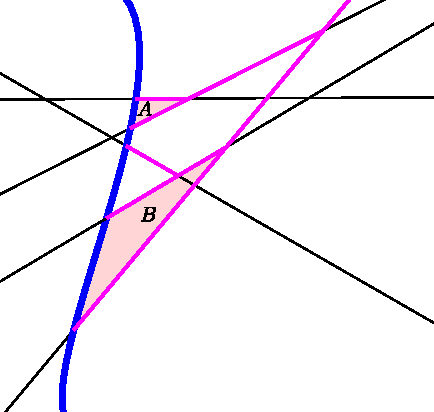
\includegraphics[height=3in]{arrangement}
    \caption{Arrangement of five lines in the plane (black lines), and a path
    (bold blue).}\label{fig:arrangement}
\end{figure}

\end{document}
